\section{SNIPER: System Description}  \label{sec:SNIPERSysDsc}
In this section we describe various components of our proposed SNIPER
framework. Figure \ref{fig:GBDSNIPER} shows the general block diagram
of the SNIPER framework where the controller interacts with Software
Defined Measurement Network (SDMN)\footnote{It must be noted that
  SNIPER does not require a separate measurement network and can be
  deployed with existing SDN-network and controller} using Network
Measurement Controlling (NMC) messages to dynamically program the SDMN
and poll the required measurements and statistics. The SDMN consists
of a set of hosts and a sub-set of OpenFlow Switches (OFS) in the
operating network. Without loss of generality, we assume that SDMN
guarantees all required IAI are \emph{observable} and
\emph{measurable}. The NMC messages include passive and active network
measurement control messages that indicate which IAI must be
accurately measured at different times and/or locations and setups
appropriate flow-table entries and probe requests in the SDMN,
accordingly. In the SNIPER framework, the network measurement process
is consisted of two stages, namely the learning and measurement
epochs, as it is shown in Figure \ref{fig:EVSmpMC}. In the supervised
learning stage the optimal IAI that must be directly measured are
precisely computed with a training data set using an evolutionary
optimization algorithm. Then, in the online measurement epoch, the the
appropriate rules are programmed in SDMN to collect the measurements
of corresponding optimal IAI. This framework can also be deployed in
dynamic environment by decreasing its dependency on the initial
training data set, instead adaptively updating the optimal observation
matrix dynamically.

%This framework can also be equipped with online EOAs where measurement and learning are concurrently performed without using the training data.
% \footnote{For optimal network monitor placement problem, please refer to \cite{LMa1:2014}, \cite{LMa2:2014} and \cite{XWang:2014}.}
%The SNIPER framework provides the ability of measuring a sub-set of the precisely chosen attributes of interest (called Optimal Network Probes (ONP)) of the operating network at different times and/or spaces which resulted in the best possible accuracy in estimating the set of all unknown attributes of interests.
\begin{figure}[t]
  \begin{center}
    {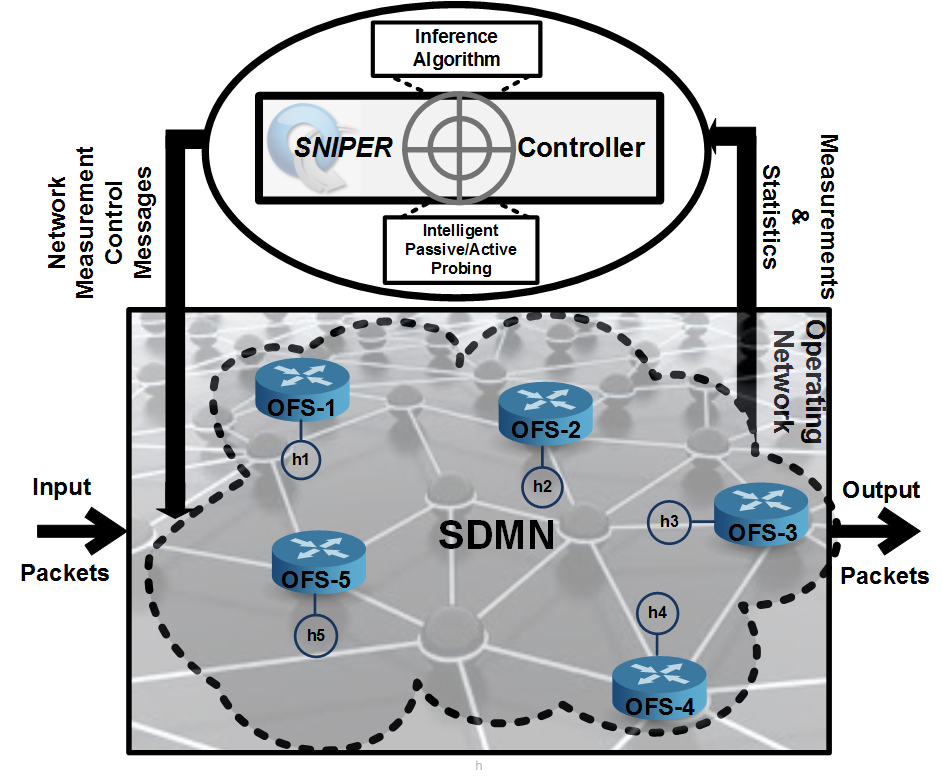
\includegraphics[keepaspectratio, width=0.49\textwidth]{GBDSNIPER_New.png}}
  \end{center}
  \caption{{SNIPER network measurement framework: a general perspective.}}
  \label{fig:GBDSNIPER}
\end{figure}
\begin{figure}[t]
  \begin{center}
    {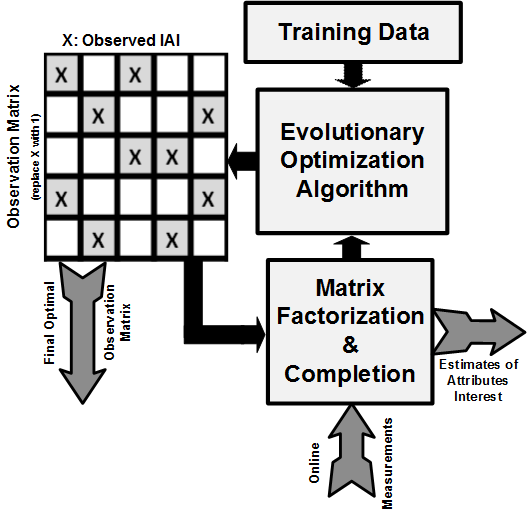
\includegraphics[keepaspectratio, width=0.35\textwidth]{EVSmpMC.png}} \\  % png
  \end{center}
  \caption{{Evolutionary optimal network probing process.}}
  \label{fig:EVSmpMC}
\end{figure}

% For passive measurement (e.g. per-flow size) the flow-tables of the SDMN is adaptively reconfigured. However, for active measurements (e.g. per-flow delay/loss) an appropriate path is first determined and flow-tables of the SDMN is adaptively reconfigured; then, probing packets are injected and routed, and required IAI are measured.
%The SNIPER controller can both preconfigure or adaptively reconfigure the flow-tables of the OFSs in SDMN. For passive per-flow size measurement, the flow-tables of the SDMN are configured and per-flow counter statistics are measured to form the matrix of per-flow sizes. In this case, ONMC messages (here, defined as passive probes) reconfigure the OFSs of the SDMN by installing different rules in flow tables and defining the required actions on the incoming packets of the operating network. 

The SNIPER controller can both pre-program or adaptively reprogram the
flow-tables of the OFSs in SDMN. For passive per-flow size
measurement, NMC messages (defined as passive probes, here)
reconfigure the OFSs of the SDMN by installing required OpenFlow rules
with appropriate forwarding actions in the flow tables for the
incoming packets. The controller also requests and collects per-flow
counter statistics to measure and reconstruct the matrix of per-flow
sizes. On the other hand, for active network performance measurements
(e.g. per-flow delay/loss/throughput), appropriate paths are first
determined (for all required entries of the matrix of IAI). Then, NMC
messages are used to actively probe the operating network by: 1)
adaptively configuring the flow-tables of the SDMN and their
forwarding actions for probing packets sent by a set of hosts; 2)
interacting with the injected probing packets into the network at the
origin of the paths, and 3) collecting required measurements at
destinations. Accordingly, the SNIPER can compute the required IAI and
obtain information of active flows and monitor the end-to-end network
performance measurements. These measurements are transmitted to the
SNIPER controller where matrix completion techniques are used as the
main NI algorithm to estimate all unknown IAI. In SNIPER, since MC
techniques only need partial measurements, not only the communication
overhead between switches and controller is low but also the amount of
network resources used for passive per-flow size measurements
(i.e. TCAM entries) and for active per-flow performance measurements
(mainly required probing bandwidth) are low.

%The measurements are transmitted to the SNIPER controller where matrix completion techniques are used as the main NI algorithm to estimate all unknown IAI. The SNIPER controller can both preconfigure the switches with forwarding rules as well as it can reactively respond to requests from switches, which are sent when a packet matches none of the existing rules enters the network. Besides managing the forwarding plane, the SNIPER controller is also capable of requesting per-flow counter statistics and injecting packets into the network. Accordingly, the SNIPER architecture can obtain information of running flows and regularly injects packets into the network to monitor end-to-end network performance measurements \cite{IF14iSTAMP:2014}\cite{Adrichen:2014}. In this framework, the communication overhead between switches and controller is low, since MC techniques only needs partial measurements. 
% In fact, under the very hard constraints of measurement resources in network monitoring applications, this framework acts as a SNIPER which precisely captures/targets the ONPs. Accordingly, the IAI can be computed because communication networks share a variety of resources of the communication infrastructure (at different layers), and accordingly, there are spatial-temporal correlations/structures \cite{Roughan:2012}\cite{YLiao:2011}\cite{Gursun:2011} that can be used by the NI algorithm to improve the estimation accuracy in inferring IAI.

The feasibility of such Software-Defined Measurement (SDM) frameworks
have been independently investigated in \cite{IF14iSTAMP:2014} and
\cite{Adrichen:2014} where the capability of OpenFlow switches can be
effectively utilized to measure and infer the IAI of the operating
network. Likewise, the SNIPER controller is capable of providing: 1)
per-flow sizes \cite{IF14iSTAMP:2014} by installing the flow ID
prefixes in the flow tables and poll the statistics; 2) per-flow
throughput \cite{Adrichen:2014} by determining specific path for each
flow and query switches to retrieve per-flow statistics where each
query determines the amount of bytes sent and the duration of each
flow; 3) per-flow packet loss \cite{Adrichen:2014} by polling flow
statistics from the first and last switch of each path and subtracting
the increase of the source switch packet counter with the increase of
the packet counter of the destination switch, and 4) per-flow delay
\cite{Adrichen:2014} by assigning a specific path to each flow and
regularly injecting packets into the first switch and having the last
switch send them back to the controller where the difference between
the packet's departure and arrival times are computed by subtracting
the estimated latency from the switch-to-controller delays. This paper
focuses on studying the performance of the SNIPER framework using two
main applications: per-flow size and delay estimations.
% For the details of the implementation please refer to \cite{IF14iSTAMP:2014} and \cite{Adrichen:2014}.
% In this paper, the performance of the SNIPER framework is mainly examined in two main applications including per-flow size and delay estimations using both synthetic and real network measurement traces from different network topologies. In addition, a prototype of SNIPER is implemented in the Mininet to demonstrate its implementation's feasibility and effectiveness.

\subsection{SNIPER: Problem Statement}   \label{subsec:ProbState}
The operating network is modeled as a connected undirected graph $G(V,E)$ where $|V|=N$, and $|E|=m$. Accordingly, there are $m$ links, and $n=N(N-1)$ paths and flows in the network, assuming that there exists an unique path between any pair of nodes in the network. As mentioned in the introduction, we model the NI problem as a Matrix Completion (MC) problem where the goal is to complete the matrix of attributes of interest ($X$) from the direct measurement of a sub-set of its entries assuming that $X$ is a low-rank matrix which contains redundancies and thus not all of its entries are needed to represent it. Here, $X$ is a matrix of size $n \times \mathcal{T}$ ($\mathcal{T}<n$) with rank $r << \mathcal{T}$ where $K$ entries of $X$ is directly measured. 
% The quantity $K$ is defined as $K=s.(n.\mathcal{T})$ where $s$ is the sampling ratio and $0 \leq s \leq 1$.
% In many network monitoring applications, the most important Internal Attributes of Interests (IAI) or performance metrics are flow size, flow throughput, packet loss and delay. Under hard resource constraints of network measurement resources (such as limited processing power and storage capacity, limited number of TCAM entries or limited bandwidth available in active loss/delay measurements) a Network Inference (NI) problem is defined as the process of estimating the IAIs based on a limited set of end-to-end or per-IAI's measurements.
% from just $O(n^{b} r log(n))$ \emph{randomly} observed entries, where $b$ is only slightly larger than 1. 

The theory of matrix completion \cite{Candes:2009} shows that under some suitable conditions, with high probability, $X$ can be exactly recovered from a set of sufficient \emph{randomly} observed entries. In practice, $X$ is often full rank but
with a rank $r$ dominant component, that is, $X$ has only $r$ significant singular values $\sigma_{1}$,..., $\sigma_{r}$ (where $\sigma_{1} \leq ... \leq \sigma_{r}$) and the others are negligible. In such cases, by minimizing the rank, a matrix of rank $r$ (denoted by $\hat{X}$) can still be found that approximates $X$ with high accuracy \cite{YLiao:2011}\cite{Candes:2009}\cite{Keshavan:2009}. Since direct minimization of the rank of a matrix is difficult, MC problems is often formulated as a convex optimization problem Eq.(\ref{MCFormu1}) where $\Omega$ is the set of observed (i.e. directly measured) entries, $P_{\Omega}$ is a sampling function that preserves entries of $X$ in $\Omega$ (i.e. $[P_{\Omega}(X)]_{ij}=x_{ij}$) and turns the others into zero, and $L(X,\hat{X}):=\sum_{i,j=1}^{n} (x_{ij}-\hat{x}_{ij})^{2}$. Corresponding to the sampling function $P_{\Omega}$, a Binary Observation Matrix $S_{\Omega}$ is also defined where $[S_{\Omega}(X)]_{ij}=1$. Accordingly, the MC searches for a low-rank matrix $\hat{X}$ that approximates $X$ with sufficient accuracy at the observed entries in $\Omega$. The unobserved or missing entries in $X$ (indicated by $\bar{\Omega}$ as the complement of $\Omega$) are predicted by the corresponding entries in $\hat{X}$. The MC problem can also be reformulated as a matrix factorization problem in Eq.(\ref{MCFormu2}) where $\hat{X}$ (with $rank(\hat{X}) \leq r$) is factorized as $\hat{X}=U_{n \times r}V_{r \times n}^{T}$ and $\lambda$ is the regularization coefficient that controls the extent of regularization. Here, the Frobenius norm of a matrix $Z$ is defined as $\left\|Z\right\|_{F}^{2}=\sum_{i,j=1}^{n} \left|z_{ij}\right|^{2}$. 

%Different methods can be used to solve optimization problem Eq.(\ref{MCFormu2}).
%The optimization problem Eq.(\ref{MCFormu2}) can be solved using different methods. 
\begin{equation}\label{MCFormu1}
%\small{
\begin{aligned}
\text{minimize} & \hspace{0.25cm} Trace \left( \hat{X} \right) = \sum_{i=1}^{n} \sigma_{i} \\
\text{s.t.} &  \hspace{0.25cm}  L\left(P_{\Omega}(X),P_{\Omega}(\hat{X})\right) \leq \delta
\end{aligned}
%}
\end{equation}

\begin{equation}\label{MCFormu2}
%\small{
\begin{aligned}
\underset{U,V}{\text{minimize}} & \hspace{0.25cm} L\left(P_{\Omega}(X),P_{\Omega}(\hat{X})\right) + \lambda ( \left\|U\right\|_{F}^{2} + \left\|V\right\|_{F}^{2} ) 
\end{aligned}
%}
\end{equation}

The optimization problem Eq.(\ref{MCFormu2}) can be solved using different methods. In this paper, we adopt two different methods from recently proposed MC procedures used in network monitoring applications to solve Eq.(\ref{MCFormu2}) and compute $U$ and $V$ matrices where $\hat{X}=UV^{T}$. The first one is the Sparsity Regularized Singular Value Decomposition (SRSVD) method \cite{Roughan:2012} that uses an alternating least squares procedure to solve Eq.(\ref{MCFormu2}). The second one is the Decentralized Matrix Factorization algorithm \cite{YLiao:2011},denoted by DMFSGD, that uses the Stochastic Gradient Descent (SGD) technique to solve Eq.(\ref{MCFormu2}). Both methods rely on the fact that the matrices of IAI in network monitoring applications contain temporal and/or spatial redundancies that can be used to estimate non-observed or missed entries.

Under hard resource constraints, it is crucial to design OOM, which leads to the best achievable estimation accuracy using matrix completion techniques. To show the importance of such a design, consider a 3$\times$3 matrix $X$ consisting of three spatial-independent processes in each row where $x_{1}(t)=\frac{1}{2}(x_{1}(t-1)+x_{1}(t+1))$, $x_{2}(t)=2x_{2}(t-1)+3$ and $x_{3}(t)=\frac{1}{2} x_{3}(t+1)-10$. Using the temporal structure in these processes, an OOM can be designed as $\Omega_{Opt}=[1, 0, 1; 1, 0, 0; 0, 0, 1]$ where there is at least one 1 in each row. Note that such an OOM can not guaranteed to be obtained using a random sampling strategy.

To maximize the performance of MC algorithms with minimum number of required measurements, such the process of designing the OOM must directly target the ultimate estimation accuracy in the network monitoring applications as defined in Eq.(\ref{NormMetrics}). However, it is extremely complicated, if it is not impossible, to formulate the MC process and target the ultimate performance criterion using a closed-form and well-defined mathematical optimization problem as a function of the observation matrix. In addition, since the observation matrix in our case is a binary matrix, it is computationally expensive and intractable to use integer optimization techniques in such a design process for large-scale networks. Therefore, in this paper, to cope with the inherent complexity of the process of designing large-scale optimal observation matrices, we apply well known evolutionary optimization algorithms that are suitable for optimization problems similar to ours.

%To maximize the performance of NI algorithms with minimum number of required measurements, such a design process must directly target the ultimate estimation accuracy in the network monitoring application. However, it is extremely complicated and computationally complex, if it is not impossible or intractable, to formulate the ultimate performance criteria using a closed-form and well-defined mathematical objective function and solve the problem using regular integer optimization techniques. Therefore, in this paper, to cope with the inherent complexity of the process of designing large-scale optimal observation matrices, we use the well known evolutionary optimization algorithms that are suitable for the optimization problems where the main objective function is a procedure or an algorithm.
%\subsection{Evolutionary-Optimal Observation Matrix Design}
%Evolutionary algorithms are the sub-category of heuristic optimization methods \cite{Talib:2009} for solving NP-hard optimization problems where the main objective function may not be formulated as a well-defined mathematical function. As Figure \ref{fig:} \cite{Kachitvichyanuku:2012} shows, evolutionary algorithms consists of three main processes. The first process is the initialization process where the initial population of individuals is randomly generated according to some solution representation. Each individual represents a solution, directly or indirectly. If an indirect representation is used, each individual must be decoded into a solution. In the second process, each solution in the population is then evaluated for a fintness value. The fitness values can be used to calculate the average population for the purpose of selection. The third process is the generation of a new population by perturbation of solutions in the existing population. The algorithm is run until one or more of the stopping criteria are met. In this paper we use two EAs namely as Genetic Algorithm (GA) and Particle Swarm Optimization (PSO) which have been applied to many optimization and machine learning problems \cite{Talib:2009}\cite{Kachitvichyanuku:2012}.
%
%The main idea of GA is to mimic the natural selection mechanism and the survival of the fittest. In GA, the solutions are represented as chromosomes. The chromosomes are evaluated for fitness values and they are ranked from the best to the worst based on fitness value. The process to produce new solutions in GA is accomplished through three genetic operators as selection, crossover, and mutation. First, the better chromosomes are selected as parents to generate new offspring (new chromosomes). To simulate the survivor of the fittest, the chromosomes with better fitness are selected with higher probabilities. Once the parent chromosomes are selected, the crossover operator combines the chromosomes of the parents to produce new offspring (perturbation of old solutions). To avoid stagnation in the process of evolution, the mutation operator is performed on the chromosomes to increase the diversity of the population. To successfully apply the GA the solution representation (i.e. chromosome model) must be designed carefully. Also, the parent selection process, and the probability of crossover and mutation are important parameters that must be precisely chosen \cite{Kachitvichyanuku:2012}.
%
%In PSO, a solution is represented as a particle, and the population of solutions is called a swarm of particles. The first process in PSO is the initialization process whereby the initial swarm of particles is generated. Each particle is initialized with a random position and velocity. Each particle is then evaluated for fitness value. Each time a fitness value is calculated, it is compared against the previous best fitness value of the particle and the previous best fitness value of the whole swarm, and, accordingly, the personal best and global best positions are updated, appropriately. If a stopping criterion is not met, the velocity and position are updated to create a new swarm. The positions and velocities of particles are updated based on the personal best and global best positions, as well as the
%old velocities. It should be noted that PSO algorithm does not require sorting of fitness values of solutions in any process. This might be a significant computational advantage over GA, especially when the population size is large \cite{Kachitvichyanuku:2012} \cite{Eberhart:2001}.
%% The velocity is updated based on three components: the old velocity (inertia or momentum term), experience of an individual particle (cognitive or self learning term), and experience of the whole swarm (group or social learning term). Each term has a weight constant associated with it.
%
%Throughout this paper, the fitness of the solutions in our evolutionary algorithms (chromosome in GA and particle in PSO) are evaluated using the following two metrics, namely, Normalized Mean Absolute Error (NMAE) and Normalized Mean Square Error (NMSE) where $x_{ij}$ denotes the $ij^{th}$ entry of the matrix $X$ (which is known in the learning stage) and $\hat{x}_{ij}$ denotes the $ij^{th}$ entry of the matrix $\hat{X}$ which is output of the MC process. 
%
%\begin{equation} \label{NormMetrics}
%\footnotesize{
%\begin{aligned}
%NMAE = \frac{\sum_{ij \in \bar{\Omega}} \left|x_{ij} - \hat{x}_{ij}\right|}{\sum_{ij \in \bar{\Omega}} \left|x_{ij}\right|} \\
%NMSE = \frac{\sqrt{\sum_{ij \in \bar{\Omega}} \left(x_{ij} - \hat{x}_{ij}\right)^{2} }}{\sqrt{\sum_{ij \in \bar{\Omega}} \left(x_{ij}\right)^{2}}}
%\end{aligned}
%}
%\end{equation}
%
%Here, a solution in the GA is represented as a chromosome which is defined as a binary sampling matrix $C$ with size $n \times \mathcal{T}$ and where $0$ and $1$ respectively represent unobserved and directly measured entries. The number of measurements paths (i.e. samples) for each chromosome is denoted by $K$ (i.e. the number of one's in each chromosome). To successfully apply the MC technique, the sampling matrix $C$ is constrained to have at least one $1$ in each row and column. The GA is started by generating $N_{p}$ chromosomes/solutions in the initialization step. Then, the fitness of each chromosome is evaluated using the cost function Eq.(\ref{NormMetrics}). Accordingly, the best chromosomes, with lowest fitness values, are selected and the crossover operation (as defined in Eq.(\ref{GACrossOver})), with probability $p_{c}$, is applied on each pair of parents to generate new children (offsprings); offsprings form the new chromosomes of the next generation. To increase the diversity of the population, the mutation operation is performed on each child where the mutation operator changes an entry of sampling matrix $C$ from zero-to-one or vice-versa with probability $p_{m}$. The GA process is continued over $N_{i}$ iterations and the best chromosome in each iteration remains unchanged.
%% Among these, the best chromosome remains unchanged; and also, some simple manipulations are applied at each step to keep the number of measurement paths constant for each sampling rate in such a way that chromosomes remain symmetric (if it is required, for example, in the case of delay measurement) with having at least an one in each row/column of $C$ (please refer to \cite{SNIPERTechReport:2014} for further details). The GA process is continued over $N_{i}$ iterations.
%\begin{equation} \label{GACrossOver}
%\footnotesize{
%\begin{aligned}
%\text{OffSpring}_{1} = C_{1}(1:r,:) + C_{2}(r+1:n,:) \\
%\text{OffSpring}_{2} = C_{2}(1:r,:) + C_{1}(r+1:n,:) 
%\end{aligned}
%}
%\end{equation}
%
%Likewise, the PSO is started by generating $N_{p}$ particles where $i^{th}$ particle is identified by its position $P^{k}_{i}$ and velocity $V^{k}_{i}$ at iteration $k$. Here, $P^{k}_{i}$ is an $n \times \mathcal{T}$ binary matrix, representing the measurement matrix, and $V^{k}_{i}$ is also an $n \times \mathcal{T}$ matrix. In the initialization stage all position and velocity matrices are zero matrices. The best position of $i^{th}$ particle obtained until iteration $k$ is denoted by $BP_{i}^{k}$ and the best position among all particles in the swarm until iteration $k$ is called global best position and it is denoted by $GP^{k}$. The best particles here is determined by evaluating the fitness of each particle and choosing the one with the minimum error value (as defined in Eq.(\ref{NormMetrics})) among all iterations (for one particle) or among all particles. 
%
%The velocity $V^{k}_{i}$ is  updated according to Eq.(\ref{PSOPosVlc}) where $c_{1}$ and $c_{2}$ are acceleration constants, which here they setup to $c_{1}=c_{2}=2$, and $\alpha_{1}$ and $\alpha_{2}$ are standard uniform random variables in interval $[0,1]$. The positive inertia weight $\omega$ is computed as  $\omega=\omega_{max}-(\omega_{max}-\omega_{min})\frac{k}{N_{i}}$ where $\omega_{min}$ and $\omega_{max}$ are respectively minimum and maximum inertia weights which, here, we setup to $\omega_{min}=0.3$, $\omega_{max}=0.9$ and $N_{i}=2000$. The particle positions are updated (by re-determining the new measurement paths) using two methods: 1) set the entries $\{p^{k}_{ij}\}_{ij\in I^{V}_{max}}=1$ where $I^{V}_{max}$ indicates the set of $ij^{th}$ entries with highest velocities in the matrix $V^{k}_{i}$ (i.e. $(\sim,I^{V}_{max}=sort(V^{k}_{i}(:))$), and 2) $\{p_{ij}\}$ is set to one with probability $sigmoid(v_{ij})$, where $sigmoid(x):=\frac{1}{1+e^{-x}}$, otherwise it is set to zero. The PSO process is continued over $N_{i}$ iterations.
%
%In both GA and PSO evolutionary algorithms, some simple manipulations are applied at each step to keep the number of measurement paths constant for each sampling rate in such a way that chromosomes/particles remain symmetric (if it is required, for example, in the case of delay measurement) with having at least an one in each row and column of the solution representation (please refer to \cite{SNIPERTechReport:2014} for further details).
%\begin{equation} \label{PSOPosVlc}
%\footnotesize{
%\begin{aligned}
%V_{i}^{k} = \omega V_{i}^{k-1}+c_{1} \alpha_{1} (BP_{i}^{k}-P_{i}^{k-1}) + c_{2} \alpha_{2} (GP^{k}-P_{i}^{k-1}) \\
%\end{aligned}
%}
%\end{equation}














%Now, if 
%
%MC techniques hagofte shavad ba tekieh bar factorization va har do raveshe mghaleha tozih dade shavad.
%
%
%moshkelat inja gofte shavad (ke rabeteii nist beine performance va strcture matrix dar resource constrainted casaes) baad dar section "`EV optimal probing design" jozeyat gofte shavad
%
%
%
% 
%the OFSs  
%
%
%
%
%
%However,
%it is a valid question to ask what the optimal observation
%(i.e. aggregation) matrix is to maximize the performance of
%CS recovery. Such a direct optimization approach for designing
%the optimal observation matrix AOpt
%g , to maximize the
%performance of CS recovery technique, is prohibitive1 due
%to the complexity of the process [24]. Therefore, to simplify
%the process of designing the optimal observation matrix other
%objective functions are considered in the optimization process,
%while accepting the unavoidable sacrifice in performance [24].
%
%
%
%
%
%  
%
%
%
%
% \cite{Candes:2009} shows that under some suitable
%conditions, with high probability, $X$ can be exactly recovered from just $O(n^{b} r log(n))$ randomly
%
%
%
%
%
%
%
%
%
%
%% \subsection{SNIPER: Problem }   \label{subsec:ProbState}
%
%
%
%that leverages the sparse or low-rank nature of real-world traffic matrices and their spatio-temporal properties to interpolate missed traffic entries due to ***
%
%\cite{Roughan:2012}
%
%SPARSITY REGULARIZED MATRIX FACTORIZATION
%
%
%
%
%
%
%
%
%
%To design and evaluate the performance of SNIPER the 
%
%% Since communication networks share a variety of resources of the communication infrastructure (at different layers), then, under the hard constraint of measurement resources, this framework acts as a SNIPER which precisely captures/targets the ONPs. 
%
%% \vspace{10in}
%%
%% to determine the best possible measurements in the next stage. This process evolves over time      
%%
%%and through an adaptive process where the Evolutionary Algorithm (EA) utilizes the statistics/measurements at each stage to determine the best possible measurements in the next stage. This process evolves over time      
%%
%% of i
%%
%%network performance quality.
%%
%%
%%
%%a variety of attributes of interest in the operating network in different time and/or spaces.  
%%
%%
%%
%%
%%
%%including per-flows sizes, link delays, packet losses and link throughputs using both passive and active probing messages. Passive messages consists of required  
%%
%%attribute of interest in SNIPER framework 
%%
%%
%%\begin{equation}\label{ISDNFMOpt2}
%%\small{
%%\begin{aligned}
%%& \hat{X} = \underset{X}{\text{minimize}} \left\|Y^{t}_{S}-HX^{t}_{g}\right\|_{p}^{2} + \lambda \left\|X^{t}_{g}\right\|_{q}\\
%%& \text{s.t.} \hspace{0.25cm} Y^{t}_{g}=A_{g}^{t} X^{t}_{g}, \hspace{0.25cm} X^{t}_{k}=A_{k}^{t} X^{t}_{k}, \hspace{0.25cm} X^{t}_{g} \geq 0\\
%%\end{aligned}
%%}
%%\end{equation}
%%
%%In iSTAMP, the communication overhead between the
%%controller and switch is low because only a few flows are
%%directly measured and other entires are used to aggregate a large
%%number of flows (hence, $T$ instead of $n$ measurement records) which is important under hard resource constraints and in multi-point measurement scenario. iSTAMP is also computationally efficient because it exploits existing low-complexity network inference techniques \cite{YCEldar:2012}.





%
%  that can not be formulated as a well-defined mathematical function.
%
%
%
%
%a closed-form and well-defined mathematical objective function that can be efficiently optimized is extremely complicated and computationally complex.
%
%The direct design of observation matrices for maximizing the performance of NI methods is prohibitive due to the complexity of the process, and therefore, to simplify the process of designing the optimal observation matrix other objective functions are considered in the optimization process, while accepting the unavoidable sacrifice in performance \cite{Elad:2007} \cite{IF14iSTAMP:2014}. The underlying difficulty in this direct optimal observation matrix design is that formulating the network inference process/algorithm into a closed-form and well-defined mathematical objective function that can be efficiently optimized is extremely complicated and computationally complex, if it is not impossible or intractable.
%
%
%
%
%Comparing to random measurement techniques used in the theory of MC, such an optimal design of the observation matrix results in 
%
%
%Under hard resource constraints of network measurement resources, the evolutionary optimization algorithms can be used to directly design the optimal observation or measurement matrix, which leads to the best achievable estimation accuracy via applying matrix completion technique onto the NI problem. Comparing to random measurement techniques used in the theory of MC, such an optimal design of the observation matrix results in 
%
%comapring to random measurement techniques This leads to the fewer or better accuracy
%
%
% how can we optimally measure or sample the entries of the matrix of attributes of interest which leads to the best possible estimation accuracy via using matrix completion techniques?}
%
%
%In the theory of matrix completion, the matrix of the attributes of interest can be completely reconstructed from a sub-set of \emph{randomly} observed entries (i.e. measurements) if the number of observations are \emph{high} enough. Accordingly, in network monitoring applications and by considering the flexibility provided by the SDN, an interesting question that can be asked is: \\
%
%\emph{
%Under hard resource constraints of network measurement resources, how can we optimally measure or sample the entries of the matrix of attributes of interest which leads to the best possible estimation accuracy via using matrix completion techniques?}
% Such an optimal measurement/observation matrix is efficient in the sense that it needs less number of measurements to reach the same estimation accuracy via random measurement scheme, or equivalently, for the same number of measurements the optimal sampling techniques reaches a better perfromance. 
%\vspace{0.15cm}\\
%
%The direct design of observation matrices for maximizing the performance of NI methods is prohibitive due to the complexity of the process, and therefore, to simplify the process of designing the optimal observation matrix other objective functions are considered in the optimization process, while accepting the unavoidable sacrifice in performance \cite{Elad:2007} \cite{IF14iSTAMP:2014}. The underlying difficulty in this direct optimal observation matrix design is that formulating the network inference process/algorithm into a closed-form and well-defined mathematical objective function that can be efficiently optimized is extremely complicated and computationally complex, if it is not impossible or intractable.
%
%Hence, in this paper and to the best of our knowledge for the first time, we change the main approach in designing the optimal observation matrix for network inference problems where we directly target the ultimate estimation accuracy in network monitoring applications in our optimization framework. However, to cope with the inherent complexity of the process of designing large-scale optimal observation matrices, we use the well known evolutionary optimization algorithms that are suitable for the optimization problems where the main objective function is a procedure or an algorithm that can not be formulated as a well-defined mathematical function.
%
% of objective functions that can not be formulated into a closed-form and well-defined mathematical 
% that the objective function can not  
%as the approximate-heuristic optimization method \cite{Talib:2009}. 
%
%\subsection{Evolutionary Algorithms (EA)}
